\chapter{Photon Detector}
\label{ch:photon}
\section{Introduction}

Liquid argon is an excellent scintillating medium. With an average energy needed to produce a photon of 19.5 eV (at zero field) a typical 1 MeV particle will generate 51,000 photons with 128 nm wavelength. At higher fields this will be reduced but at 500 V/cm the yield is still $\sim$40,000? %\fixme{What's with the ? Russ says to leave it for now. 1/5/15} 
photons per MeV. Roughly 1/3 of the photons are prompt 2-6 ns and 2/3 are generated with a delay of 1100-1600 ns. LAr is highly transparent to the 128 VUV photons with a Rayleigh scattering length and absorption length of 95 cm and >200 cm respectively. The relatively large light yield makes the scintillation process an excellent candidate for determination of $t_{0}$ for non-beam related events. Detection of the scintillation light may also be helpful in background rejection.

\section{Requirements and Goals}

\subsection{Beam-based physics}

There are no requirements for the beam-based physics program, as the machine clock will provide a $t_{0}$ with roughly 10 $\mu$s resolution. Given that the electron drift is 1.6 mm/$\mu$s the uncertainty to the electron lifetime correction is small is the beam timing is used. The photon system can be useful in determining the $t_{0}$ of cosmic ray events and events from radiological decays. The impact of this on the detector performance needs to be determined, but it is not expected that the reduction in backgrounds for the oscillation program will introduce additional requirements to the photon system design.


\subsection{Proton decay and atmospheric physics}

The photon detector system must provide the t0 for non-beam related physics channels if a correction for electron recombination during drift is to be applied. The requirements for electronics and hadronic energy resolution for the proton decay and the atmospheric neutrino program are $1\% / \sqrt{E(GeV)} \bigoplus 1\%$ and $30\% / \sqrt{E(GeV)}$  respectively. With these resolutions the collected charge must be accurately corrected for recombination. Therefore the photon system must provide a $t_{0}$ for particles with >100 MeV with >95\% efficiency in the fiducial volume of the detector. 


\subsection{Low-energy physics}

Supernova events will produce neutrinos down to about $\sim$5 MeV. Studies have estimated the momentum resolution for 5 MeV electrons to be 20\% using only TPC information and assuming a highly efficient trigger and an electron lifetime of 5 ms. The impact of various detector resolutions on the physics potential of LBNE has not been studied in detail. At present there is no strong requirement that the energy resolution must be better than 20\% so no requirement on the photon system trigger efficiency is set at this time. However it is clear that if a detector design can be found the energy resolution would greatly improve. A goal of the photon detection R\&D is to develop a system with the lowest possible threshold for a reasonable cost. At time of the start of final design a final decision as to the configuration will need to be made based on cost and added physics capability.

\subsection{General Considerations}
In the event that larger photon collection efficiencies can be achieved then it is possible to improve the energy resolution of the detector by adding the photon yield to the electron yield information.  However this requires several orders of improvement in light collection efficiency so it is beyond the scope of present designed.

\section{Cast or Bulk doped acrylic bars}

The reference design for the photon detection system is based on acrylic bars, which are either coated in TPB or doped in bulk. The 128 nm photons interact with the TPB on the surface and 430 nm light is re-emitted. 

A PD module is made up of 4 light guides that capture, waveshift, and channel VUV photons to silicon photomultipliers (SiPMs) at one end.  A schematic drawing of a cast acrylic light guide with its photosensors is shown in Figure~\ref{fig:cast-acryl-lightguide}.

\begin{figure}[htbp]
\centering
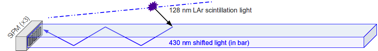
\includegraphics[width=.6\textwidth]{cast-acryl-lightguide}
\caption[Schematic drawing of cast acrylic light guide]{Schematic drawing of cast acrylic light guide with associated photo-sensors}
\label{fig:cast-acryl-lightguide}
\end{figure}


The light guides are made from cast acrylic bars that have wavelength shifter embedded in them.  The wavelength shifter converts VUV scintillation photons striking it to 430 nm photons inside the bar, with an efficiency of ~50\% of converting a VUV to an optical photon.  A fraction of the waveshifted optical photons are internally reflected to the bar's end where they are detected by SiPMs whose QE is well matched to the 430 nm waveshifted photons. The light guides were made with one of two wavelength shifters: the conventional TPB (1,1,4,4-tetraphenyl-1,3-butadiene) and the less expensive alternative bis-MSB (1,4-bis-(o-methyl-styryl)-benzene). Preliminary studies with a VUV monochromator show that the two wavelength shifters compare favorably in their waveshifting efficiency.  
Several technologies have been investigated at Indiana University for incorporating the waveshifter into the acrylic (or in one case, polystyrene), including:  

1.  Flash heated bars

These light guides were made with TPB and bis-MSB using commercially available Lucite-UTRAN cast UVT acrylic sheet that was laser-cut into bars of the proper size. Lucite-UTRAN has an attenuation length of 2.5 m.  To embed the WLS in the acrylic, the bars coated with waveshifter are flash heated to rapidly melt the WLS into a thin outer layer of the bar. 

2.  Hand-dipped bars

These light guides were made by dip-coating acrylic bars in a WLS solution, a process that was pioneered at MIT.  This process improves the clarity and uniformity of the coating, as well as its scalability to the manufacture of the large number of light guides needed for LBNE.  In this process, a solution is mixed with 2 parts TPB/bis-MSB to 100 parts DCM (dichloromethane, $CH_{2}Cl_{2}$).  Each acrylic bar is submerged in this solution, removed, and then left to air dry.

3.  Doped, cast acrylic bars

These light guides were cut from a sheet of acrylic cast with TPB or bis-MSB mixed into the plastic. This sheet was manufactured commercially by Astra Products, Baldwin, NY.  The sheet had 1\% TPB or bis-MSB by mass added during their proprietary casting process, which distributes WLS throughout the volume.  Experiments show that 1\% WLS is the maximum that can be cast into the plastic without particles settling out.  Since VUV photons have a very short penetration depth in acrylic, this manufacturing method uses more WLS than necessary.  On the other hand, light guides function more efficiently when their surfaces are flat and the casting process results in very flat surfaces.  This is a strong mitigating factor when the prime consideration is efficiency for the detection of VUV photons. 

4.  Doped, cast polystyrene

These light guides are made commercially by Eljen Technologies, a `'world leader in the development and manufacturer of organic plastic scintillation material.''  These light guides were cut from a sheet of polystyrene cast with TPB or bis-MSB mixed into the plastic by a proprietary process.  The sheet had 1\% TPB or bis-MSB by mass added during their proprietary casting process, which distributes WLS throughout the volume. 
 
In addition to these designs a thin bar (or fiber) with dimensions 3 mm by 3 mm was developed by the CSU group. The square profile fiber-based prototype design was motivated by the fact that 4 fibers would exactly couple to the 6 mm by 6 mm active area of the SiPM currently under consideration for the photon detector system. The fiber size allowed 100\% areal acceptance to SiPM mapping, within efficiencies associated with photon conversion and transport. The fibers used in the prototype were custom fibers made by St. Gobain with a concentration of 1\%, by weight, of TPB mixed into the bulk during manufacture.   

\subsection{Current status of design}

The designs have been tested at two facilities, the local LAr at Indiana University and at the TallBo dewar in lab PAB at Fermilab.  The light guide designs are tested in a PD paddle frame designed and built at Colorado State U that holds 4 light guides.  

Selected Results from IU dewar facility

\begin{figure}[htbp]
\centering
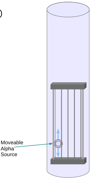
\includegraphics[width=.3\textwidth]{iu-dewar-paddle-frame}
\caption{IU dewar paddle frame showing movable alpha source}
\label{fig:iu-dewar-paddle-frame}
\end{figure}

The IU dewar shown in Figure~\ref{fig:iu-dewar-paddle-frame} below can hold 1 paddle.  The IU dewar tests can be used for both studying cosmic muons and attenuation length measurements with a $^{241}$Am $\alpha$ source.  For the setup shown in Fig. 2, the $^{241}$Am $\alpha$ source is moved up the light guide and a set of waveforms are collected every 2 inches.  The distribution of the waveforms collected at each of the 10 positions for a hand-dipped bar with TPB is shown in the left side of Figure~\ref{fig:waveforms-and-fit}.  The individual photoelectron peaks are clearly visible.  The peak of the distribution nearest the SiPM is approximately 30 pe's.  At the farthest point, the peak is approximately 15 pe's.  The distributions have all been  normalized to have the same area.  Since the standard deviation of the waveform distribution nearest to the SiPM are larger than those farther away, the near distributions are less peaked and wider. 

The distribution of waveforms at each position along the bar is shown in the right side of Figure~\ref{fig:waveforms-and-fit}.  Superposed is an exponential fit to the peak of these waveform distributions.  This fit shows that the attenuation length of the bar is $\sim$37 inches, the longest attenuation length yet seen for the light guide technology. 
\begin{figure}[htbp]
\centering
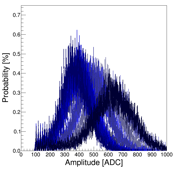
\includegraphics[width=.4\textwidth]{stacked-waveforms}
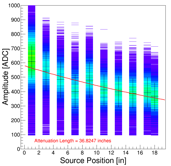
\includegraphics[width=.4\textwidth]{single-exp-fit}
\caption{Left: Stacked waveforms for 11 positions of the $\alpha$ source along the bar. Right: The results of fitting a single exponential to the measurements on the left.  The attenuation length is $\sim$37 inches. }
\label{fig:waveforms-and-fit}
\end{figure}


There were 3 bars made in this batch of hand-dipped bars.  One of those bars had an attenuation length of $\sim$31 inches, comparable to this result.  One, however, had an attenuation length of $\sim$14 inches  It will be one of the objectives of next year's R\&D efforts to understand how to make light guides with consistently long attenuation lengths. 
 
Selected Results from the TallBo dewar facility

The TallBo dewar facility at Fermilab is described more fully in section 2.8.1.  It is a 450 liter dewar in lab PAB at Fermilab.  It is large enough to hold 4 full PD paddle frames loaded with 20-inch light guides.  The TallBo dewar recirculates the LAr and maintains its purity for weeks at a time.  It is the test facility we use at IU for longer-term comparison  studies of many alternative technologies.  
The IU group has run two experiments at TallBo so far, one in October-November 2013 and one in February-March 2014.  The goal of these experiments was to make inter-comparisons of several light guide technologies under uniform conditions.  In order to correct these comparisons for systematic effects, we constructed a Monte Carlo simulation of the experiment.  First we made a model of the light guides; then we put this model into a full simulation of the TallBo dewar; finally, we tracked scintillation photons generated by cosmic muons to the light guides, into the light guides, and then down the light guides to the SiPMs.  

The light guides were modeled as 20-inch acrylic bars with waveshifter embedded in their surfaces that convert 128 nm photons from LAr scintillation light to 430 nm light in the bar.  The simulation then propagates the optical photons to the SiPMs at the end of the bar.   The left side of Figure~\ref{fig:mc-sim-and-tallbo}. shows the results of one such simulation in which the waveshifted light has been separated into the fraction of the total that propagates directly to the SiPMs and the fraction that is internally reflected to the SiPMs.  Near the SiPM a significant fraction of the light propagates directly to the photodetectors.   After 5-10 cm, the light comes mostly from internally reflected light.  

\begin{figure}[htbp]
\centering
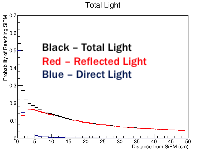
\includegraphics[width=.42\textwidth]{mc-sim-420nm}
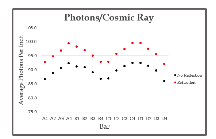
\includegraphics[width=.42\textwidth]{light-inc-tallbo}
\caption{Left: Monte Carlo simulations of the 420 nm light seen by the SiPMs as a function of distance along the bar. Right: Increase in the light due to reflections in the TallBo dewar for the different light guide technologies. }
\label{fig:mc-sim-and-tallbo}
\end{figure}

\begin{figure}[htbp]
\centering
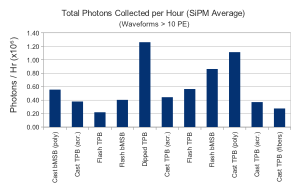
\includegraphics[width=.7\textwidth]{total-photons-per-hr}
\caption{Comparison of several light guide technologies including the CSU fiber technology in the TallBo dewar.  The corrections for systematics in Figure~\ref{fig:mc-sim-and-tallbo} (right) have been applied. }
\label{fig:total-photons-per-hr}
\end{figure}


The TallBo simulation was designed to answer two basic questions.  The first of these questions is the way in which reflected light from the stainless steel walls Figure~\ref{fig:total-photons-per-hr} affects the measurements.  The results of that study are shown in the right side of Figure~\ref{fig:mc-sim-and-tallbo}.  Both the geometric corrections (black circles) and the corrections due to reflections (red circles) have been applied to the data.
The results of the comparisons for 11 light guides made with 8 different technologies, including the prototype fiber light guide from CSU, during the February-March 2014 TallBo run are shown in Fig. 7.  What seems to be clear  from Fig. 7 is that the dipped technology pioneered by the MIT group has a better response than the flash heated bars manufactured by the technology developed at IU.  After these results were obtained we have moved away from the flash heated technology and invested our R\&D efforts into our development of the dipping technology.  These results have also motivated the CSU group to modify their fiber design and produce a substantially improved prototype fiber light guide. 








